\section{Results}
\begin{table}[h!]
\begin{tabular}{ c | c | c |  c | c | c | c |  c | c | c |  c }
 ~chr1.fa & ~chr2.fa  & ~chr3.fa & ~chr4.fa & ~chr5.fa & ~chr6.fa &  ~chr7.fa & ~chr8.fa & ~chr9.fa & chr10.fa & chr11.fa \\
 \hline
246.284 & 242.003 & 198.723 & 190.526 & 180.152 & 170.233 & 158.202 & 145.704 & 139.726 & 134.846 & 133.928
\end{tabular}
\begin{tabular}{ c | c | c |  c | c | c | c |  c | c | c |  c }
chr12.fa & chr13.fa & chr14.fa & chr15.fa & chr16.fa & chr17.fa & chr18.fa & chr19.fa & chr20.fa & chr21.fa & chr22.fa\\
\hline
131.833 & 113.698 & 105.954 & 99.947 & 88.481 & 78.468 & 75.820 & 63.563 & 62.193 & 46.761 & 49.498
\end{tabular}
\caption{Fasta files from http://hgdownload.cse.ucsc.edu/goldenPath/hg18/chromosomes/ with sizes in KB}
\label{tab:sizes}
\end{table}
Looking at Table~\ref{tab:sizes}, we have a series of fasta files, ranging from 246.284KB to 46.761 KB in size, each fasta file has a number, and besides $chr22.fa$, every number is decreasingly lower in size as to the previous.

\begin{figure}[h!]
\centering
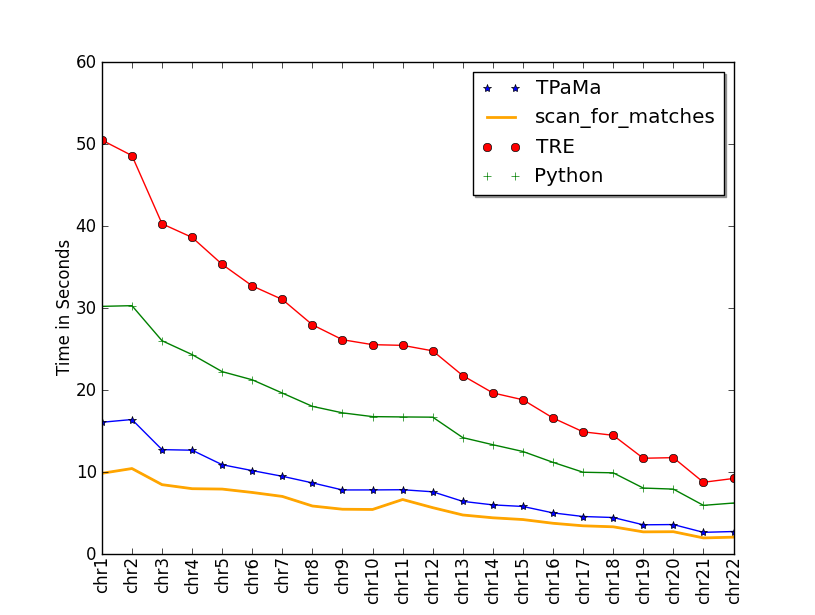
\includegraphics[width=0.6\textwidth]{Benchmarking/1ins.png}
\caption{Running time of search through fasta files mentioned in Table~\ref{tab:sizes},  allowing one insertions on pattern TGCAAGCGTTAAT}
\end{figure}

\begin{figure}[h!]
\centering
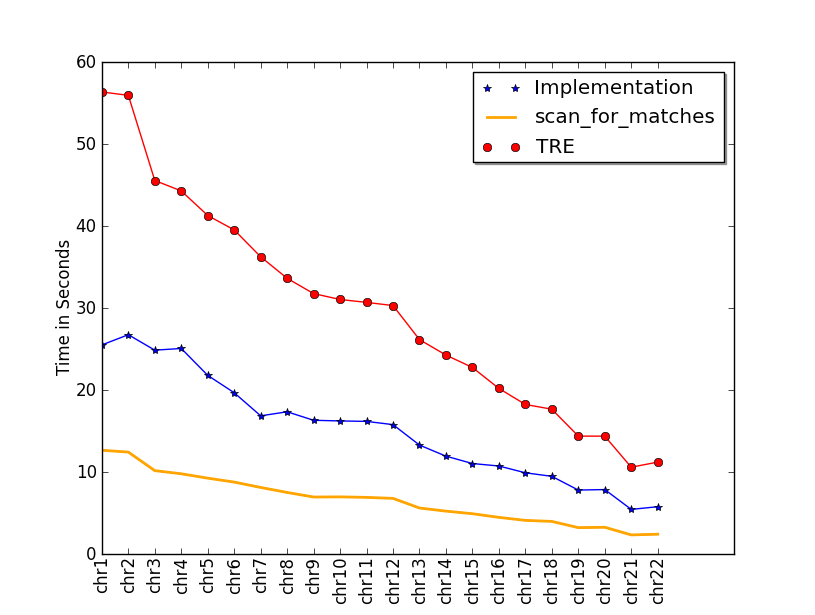
\includegraphics[width=0.6\textwidth]{Benchmarking/2ins.png}
\caption{Running time of search through fasta files mentioned in Table~\ref{tab:sizes},  allowing two insertions on pattern TGCAAGCGTTAAT}
\end{figure}
